\documentclass[a4paper, 12pt, one column, aas_macros]{article}

%% Language and font encodings. This says how to do hyphenation on end of lines.
\usepackage[english]{babel}
\usepackage[utf8x]{inputenc}
\usepackage[T1]{fontenc}
\usepackage{aas_macros}
\usepackage{url}
\usepackage{url}

%% Sets page size and margins. You can edit this to your liking
\usepackage[top=1.3cm, bottom=2.0cm, outer=2.5cm, inner=2.5cm, heightrounded,
marginparwidth=1.5cm, marginparsep=0.4cm, margin=2.5cm]{geometry}

%% Useful packages
\usepackage{graphicx} %allows you to use jpg or png images. PDF is still recommended
\usepackage[colorlinks=False]{hyperref} % add links inside PDF files
\usepackage{amsmath}  % Math fonts
\usepackage{amsfonts} %
\usepackage{amssymb}  %

%% Citation package
\usepackage[authoryear]{natbib}
\bibliographystyle{abbrvnat}
\setcitestyle{authoryear,open={(},close={)}}


\title{
Stats 4M03 Final Project \\
\large Mammogram Mass Data Analysis
}
\author{Sara Awid}




\begin{document}
\maketitle

\section{Introduction and Background}
	Mammography is the most effective method for breast cancer screening
    available today. However, the low positive predictive value of breast
    biopsy resulting from mammogram interpretation leads to approximately
    70\%  of unnecessary biopsies with benign outcomes \citet{MMA}.  Normally, physicians interpret the mammogram results based on the visual aspects of the lesion mass shape, density (the amount of fat cells present and density of suspicious cells), and its margin (the margin of benign lesion is well defined). To reduce the high
    number of unnecessary breast biopsies, several computer-aided diagnosis
    (CAD) systems have been proposed in the last years. These systems
    help physicians in their decision to perform a breast biopsy on a suspicious
    lesion seen in a mammogram or to perform a short term follow-up
    examination instead \citet{MMA}. We would like to see how significant the  CAD system which in our case is called BI-RAD (Breast Imaging and Reporting Data System) assessment preforms as a classifier against a physician interpretation. In our data, the severity (benign or malignant) of a mammography mass  is determined from BI-RADS attributes and the patient's age. \\




\subsection{Data Description}    
     The mammographic mass dataset of clinical breast cancer cases
was obtained from the Mammographic Mass Database
available in the UCI Machine Learning Repository.  \citet{MMA}.The data was collected at the Institute of Radiology of the University Erlangen-Nuremberg between 2003 and 2006. Below is the breakdown of the attributes in the dataset. The range of each attributes affect essentially the severity of the tumor. For example, higher values of BI-RADS indicate suspicious tumor. Any irregular shape or ill defined margin and higher density can indicate signs of suspicious mass.
\\



\begin{enumerate}
  \item BI-RADS assessment: 1 to 5 (ordinal)
  \item Age: patient's age in years (integer)
  \item Shape: mass shape: round=1 oval=2 lobular=3 irregular=4 (nominal)
  \item Margin: mass margin: circumscribed=1 microlobulated=2 obscured=3 ill-defined=4
  \item Density: mass density high=1 iso=2 low=3 fat-containing=4 (ordinal)
  \item Severity: benign=0 or malignant=1 
\end{enumerate}  

\subsection{Data Cleaning}
In total we have 961 of instances consisting of  516 benign and 445 malignant tumors. However, there are several instances of missing data which are outlined in the table below. The missing data were entered as a question mark "?". After eliminating all the rows with missing data, we had 830 rows, so we lost approximately 13 \% of the data. 

\begin{center}
\title Meta Data Breakdown Before Data Cleaning and Filtering 961 rows
\\
 \begin{tabular}{||c c c c c ||} 
 \hline
 Role & Name & Type  & Range & Missing Data\\ [0.5ex] 
 \hline\hline
 Label& Severity & Binomial & 1, 0 & 0 \\ 
 \hline
Regular & BI-RADS & Nominal & 1-5 & 2 \\
 \hline
 Regular & Shape & Nominal & 1-4&31 \\
 \hline
Regular & Margin & Nominal & 1-4&48 \\
 \hline
Regular & Density & Nominal & 1-4&76 \\
\hline
Regular & Age & Nominal & 18-96&5 \\ [1ex] 
 \hline
\end{tabular}
\end{center}

\subsection{Relevant Background}
In the next sections we will discuss some of the data analysis techniques we have learned in class.We will classify the data using Decision Trees to see how we can classify the tumors based on the given attributes and  we will use Logistic Regression to see which of the attributes are significant and how does BI-RADS rank. Finally, we will use Principal Component Analysis to see how many PC's we can use.   

\begin{itemize}




\item \textbf{Classification Tree }  a method to help us classify and predict the value of a target (or dependent variable) based on the values of several input (or independent variables).

\item \textbf{Binary Logistic Regression }  is a special type of regression where binary response variable is related to a set of explanatory variables, which can be discrete and/or continuous. It estimates the probability that a characteristic is present (e.g. estimate probability of "success") given the values of explanatory variables.
\\
Let Y be a binary response variable, i.e.
Yi = 1 if tumor malignant for person i and Yi = 0 if tumor benign  for person i. Let X = (X1, X2, ..., X5) be a set of explanatory variables which can be discrete, continuous, or a combination. Xi is the observed value of the explanatory variables for observation i. Then, to to predict the probability that a given example belongs to the “1” class versus the probability that it belongs to the “0” we use the following probability model expression:

$E[Y | x]=P[Y = 1 | x]=\pi(x)= \frac
	{exp\left \{ \beta _{0} + \beta _{1}x  \right \}}
	{1+exp \left \{ \beta _{0} + \beta _{1}x \right\}}
$
\citet{MCN2}
\item \textbf{Principal Component Analysis}
is a procedure for identifying a smaller number of orthogonal variables, called "principal components", from a large set of data. The goal of principal components analysis is to explain the maximum amount of variance with the fewest number of principal components. Thus, for r > 1: the ith principal component is the direction of most variation
(in the data) conditional on it being orthogonal to the first i − 1
principal components. Let X be a p-dimensional random vector with mean $\mu$ and covariance
matrix $\sum$.
Then, the ith principal component of X is
Wi = v′
i(X − µ),
for i = 1,...,p which we can be written as
W = V′
(X − µ),
where W = (W1,...,Wp)′ and V = ($\nu_{1}  \nu_{2} \cdots \nu$). Let  $\lambda_{1}  \geq  \lambda_{2} \geq\cdots \geq  \lambda_{p} \geq  0 $ be the 
eigenvalues of $\Sigma$ , and let
$\nu_{1},  \nu_{2} \cdots \nu$ be the corresponding eigenvectors. Then, the proportion of the total variation explained by the ith principal
component is $\frac{\lambda _{i} }{tr{\Sigma }}$ and the proportion of the total variation explained by the first k principal components is $\frac{\sum_{i=1}^{k} \lambda _{i} }{tr{\Sigma }}$ \citet{MCN}


\end{itemize}

\section{Classification Tree}


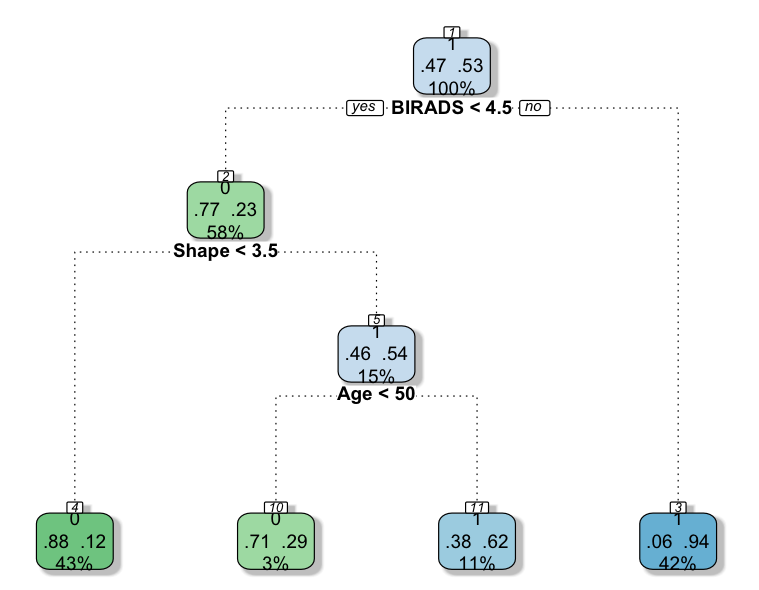
\includegraphics[width=\textwidth]{Classification_Tree2.png}
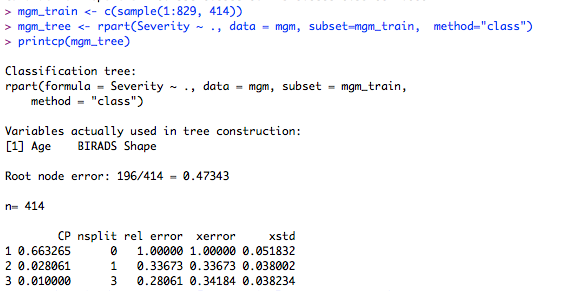
\includegraphics[width=12cm]{Classification_Tree.png}
\\	The first step we did is we took 414 random data points as sample from the Mammogram data. This was our training dataset. We ran the classification tree algorithm on the training data.
The algorithm starts at the top and looks at the whole training data set and recursively partitions the data based on the best splitter. At each split, the decision tree create a node, the algorithm chooses a split that minimizes the MSE of predictions compared to the training data. Once the algorithm cannot split the data into further nodes, it reaches a terminal node.
The output of this algorithm is the classification tree above and it splits based on the rate of BI-RAD assessment, if it is greater than 4.5, then it is determined that 42\% of the tumors are expected to be malignant while the other 58\%  (tumors with BI-RAD less than 4.5) are going to have severity determined based on the next two nodes, Age and Shape. If the shape is less than 3.5, ie, round or oval, then we expect the tumor to be benign, which is 43\% of our data structure. However if the shape is not oval or round, then the tumor can be classified based on the age. If the patient has a tumor that is neither round nor oval and is over 50 years old, then we predict the tumor to be malignant, 11\% of our patients met these criteria. Otherwise, under the same shape criteria, if the patient is less than 50 years old then 3\% of tumors were predicted to be benign. \\
\\Nevertheless, there are misclassification in our decision tree, if you look at the 4th terminal node, 88\% of tumors were classified correctly as benign while the other 12\% were classified as benign when in fact they were malignant. The Shape node here failed to classify some round or oval mass as malignant, which essentially is difficult to classify since these shapes are of a benign mass normally, but unfortunately this is a serious misclassification if biopsy was determined unnecessary. Similarly in the tenth node, 29\% of patients who did fall under this node were misclassified as benign when they actually are malignant, while 71\% were classified correctly. In the eleventh terminal node, we see the poorest classification rate, out of the 11\% instances, 38\% of masses were classified as malignant when they are benign, and the remaining 62\% were classified as malignant correctly. In the rightmost third terminal node, the classification rate was the best as we have only 6\% of the 42\% instances being misclassified as malignant and the remaining 94\% classified correctly.\\
\\The table above is the output of the decision  \textit{printcp} function which gives cross-validation estimates of misclassification error (xerror), standard errors (xstd) of those estimates and the training (re substitution) estimates (error). We can see that a 3 CP split rate gives the smallest relative error. We can also conclude that out misclassification rate is approximately 13\% when we look at the relative error* the root node error=0.47343* 0.28061=0.1328492. Additionally, if we look at the prediction table below, we see that our classification does contain 30 instances in which benign masses were classified as malignant and 44 malignant were classified as benign. In conclusion, despite the misclassification instances we get using our classification tree, we can see that using the BI-RAD and other attributes are by far better classifiers than a radiologist mammogram interpretation that results in misclassification rate of 70\% on average.
\\
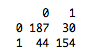
\includegraphics[width=4cm]{PredictorTable.png}
\\

\section{Binary Logistic Regression} 
The first step here is splitting the data into two chunks of test and training data as we did similarly above in the classification tree algorithm. We then fit the model using the training data to see which predictors are significant in estimating the severity of the mass. The output (\textit{model}) shown below indicates that BIRADS, Age, Shape are more significant, while mass Density and Margin are not significant predictors (p-value is greater than 0.05). Indeed, the model suggests a very strong relationship between BIRADS and the Severity of the mass as expected. Furthermore, this result is consistent with our classification tree algorithm which splits the data based on the same significant logistic regression predictors.\\
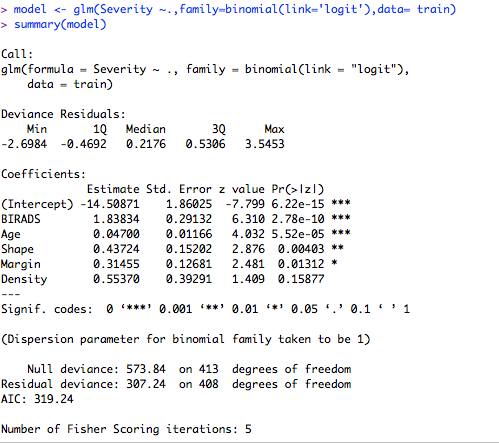
\includegraphics[width=\textwidth]{Regression_Summary.png}
\\The next thing we want to explore is the analysis of deviance to understand further which predictors we could possibly collapse using the likelihood ratio test. In our model output above, G= D(model without the variable) − D(model with the variable)=-537.84-307.24. G$\sim 
\chi ^{2}$= 7.95411e-48 . The null hypothesis (a model with only the intercept)is that the more complicated model is no better; we therefore reject the null hypothesis.\\
\\Additionally, if we look at the Analysis of Deviance Table below, we see that the difference between the null deviance and the residual deviance shows how our model is doing against the null model. In Deviance column, we can see the drop in deviance when adding each variable one at a time. Again, the BIRADS, Age and Shape drop the residual deviance significantly, while Margin and Density have higher p value which indicates that the model without these two variables explains more or less the same amount of variation. 
\\
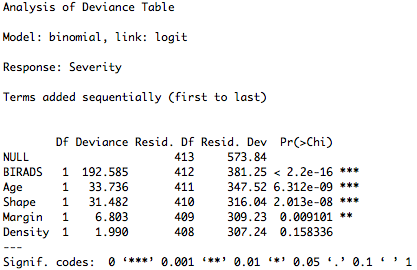
\includegraphics[width=10cm]{ChiTest.png}
\\Finally, we will assess the performance of our binary classifier using the ROC curve. A ROC curve is a plot of sensitivity (y-axis) versus specificity, or 1 – specificity, (x-axis). Below is the plot of the ROC curve indicating the trade off between sensitivity (the proportion of events correctly predicted as events (true
positives)) and specificity (the proportion of non-events correctly predicted as non-events (true negatives)). In other words, the true positive rate is basically how often does the classifier predict positive when the actual classification is positive (meaning malignant). The false positive  how often does the classifier incorrectly predict positive when the actual classification is negative (meaning benign). \\
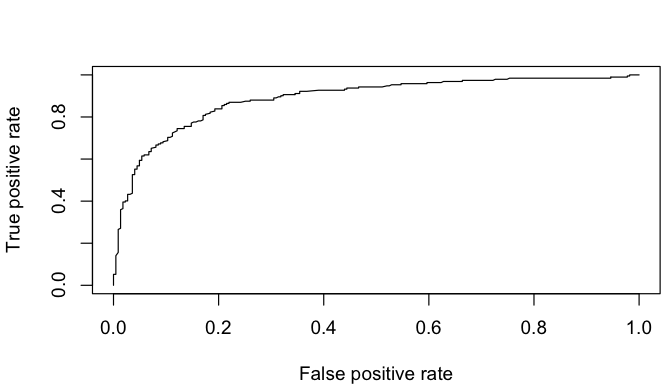
\includegraphics[width=10cm]{RocCurve.png}
\\
As we can observe from the plot, the ROC is skewed to the top left which indicates that our classifier is going to rank true positive rates probability higher than a false positive probability. The area under the curve is calculated to be 0.887799 which is a good indication for how well our classifier is doing. \\
\section{Principal Component Analysis}
Principal component analysis is a data reduction technique used when variables are highly correlated. In our dataset, shape, margin and density for a mass can be correlated when the tumor depicts strong characteristics when it is either malignant or benign. The output of the PCA below shows us that the first PC loads negative with an even range of 43\%-56\% on all predictors with the exception Density as it loads significantly lower than the rest.  The second PC loads exceptionally heavily on density with -98\% while the remaining variables are loading positively less than 0.1. The summary table below is indicating the total and proportional variation each PC has. We can see that the first and second PCs explain 47.7\% and 67.47\% of the variation in the data, therefore it is safe to conclude that the first two PCs explains the majority of the data. The plot of the variations vs the number of PCs also shows the bend in the plot at the second PC in which any addition of PC will have a small marginal effect on the variation explained by the data. 
\\
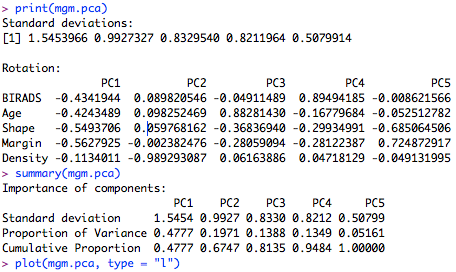
\includegraphics[width=10cm]{PCA.png}

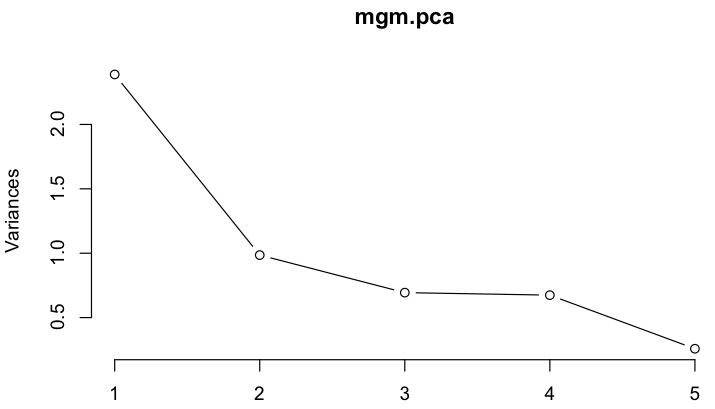
\includegraphics[width=10cm]{PCAplot.png}




\section{Summary and Conclusion}
Based on our analysis above, we conclude that the proposed computer aided system BI-RADS assessment along with other attribute of the patients age can help radiologist determine the severity of the mass by providing a more accurate classification rate and thus recommend a biopsy when necessary. The classification rate is significantly better than 30\% success rate radiologist obtain based on mammography interpretation alone. The classification tree algorithm did a fair job in splitting the data based on the BI-RAD assessment and further based on the shape and age of the patient. Similarly, we tested the significance of the attributes as predictors and concluded to the same result that BI-RAD, Shape and patients age are indeed significant in assessing the severity of the mass while margin and density are not as significant predictors.This result was also consistent with our analysis of deviance as we showed that density and margin have high p-values and thus can be dropped from our model and we would obtain similar results. As a bonus, we looked at the ROC curve and tested how well the binary classifier preforms and we had a good AUC that indicated higher ranking to true positives than false positives. Finally, PCA shows that we can get away with using only two PC as they explain the highest variation in the data.      












 \pagebreak
\bibliography{refs}
\end{document}